	\begin{center}
		\section{数论}
	\end{center}

	\begin{multicols*}{2} % 开始双栏，数字 2 表示分两栏

		\subsection{线性筛}

		\href{https://www.notion.so/3224539447bd8073af5bddda3976d8ca?pvs=21}{完全理解线性筛} \\

		线性筛的作用就是为了保证每个合数都只被其【最小的】那个质因数标记一次。

		对于一个将被标记的合数，我们记为 $h$。在遍历过程中，它由当前的数字 $i$ 和枚举到的素数 $p$ 相乘得到：
		$$ h \leftarrow i \times p $$
		线性筛的核心要求是，我们希望 $p$ 恰好是 $h$ 的最小素因数。

		假设将 $i$ 分解素因数，其分解形式为 $i = p_{i1} \times p_{i2} \times \dots$，其中 $p_{i1}$ 是 $i$ 的最小素因数，也就是代码中记录的 \verb|minp[i]|。
		那么合数 $h$ 的因数分解可以表示为：
		$$ h \leftarrow \underbrace{(p_{i1} \times p_{i2} \times \dots)}_{i} \times p $$

		为了使 $p$ 确实是 $h$ 的最小素因数，必然要求 $p \le p_{i1}$，即要求：
		$$ p \le \text{minp}[i] $$

		因此，在线性筛的内层循环中（\verb|for p in primes|），我们首先执行：
		\begin{minted}{cpp}
minp[i * p] = p;
		\end{minted}

		当遇到满足 \verb|p == minp[i]| 的情况时，说明当前的素数 $p$ 已经达到了 $i$ 的最小素因数边界。
		由于 \verb|primes| 列表是递增的，如果继续往后枚举素数，后面的素数必定严格大于 \verb|minp[i]|，这样新枚举的素数就不再是所生成合数（$i \times p'$）的最小素因数了。
		因此我们必须在此处执行 \verb|break|，从而保证每个合数仅被其最小素因数筛除。

		\href{https://qoj.ac/submission/995868}{qoj 995868}

		\href{https://cp-algorithms.com/algebra/prime-sieve-linear.html}{cp-algorithms 线性筛}

		\begin{minted}{cpp}
//  minp[i] 存储的是i的最小素因数
// https://www.luogu.com.cn/record/221554377
vector<ll> minp,primes;
void sieve(ll n){
	minp.resize(n+5);
	// minp[1]=1;  // 加了这句话可能把 1 误判成素数，要小心
	for(int i=2;i<=n;++i){
		if(minp[i]==0){		// 是素数
			minp[i]=i;
			primes.push_back(i);
		}
		for(auto p:primes){
			if(i*p>n){	// 超范围了
				break;
			}
			minp[i*p]=p;
			// 为了保证每个合数都只被其【最小的】那个质因数标记一次 break
			if(p==minp[i]){
				break;
			}
		}
	}
}

// 沿 minp 拆出 n 的素因子列表（计重）；长度=Omega, sort+unique 后=omega
vector<ll> pFacLs(ll n) {
	if (n <= 0) return {};
	vector<ll> pLs;
	while (n != 1) {
		pLs.push_back(minp[n]);
		n /= minp[n];
	}
	return pLs;
}
		\end{minted}

		使用线性筛的minp分解素因数更快，效率更高。用法（如 CF2238D，答案 $\Omega+\omega-1$）：

		\begin{minted}{cpp}
	vector<ll> pLs = pFacLs(N);					// 素因子列表（计重）
	ll pCt = pLs.size();						// Omega = 列表长度
	sort(all(pLs));
	ll sz = unique(all(pLs)) - pLs.begin();		// omega = 去重后长度
		\end{minted}

		\subsection{Miller-Rabin 与 Pollard's Rho}

		模板题：\href{https://vjudge.net/problem/洛谷-P4718}{洛谷 P4718【模板】Pollard-Rho}（\href{https://vjudge.net/solution/69880751}{AC 提交}）。

		\verb|is_prime(n)| 用前 7 个固定底数做确定性 Miller-Rabin，覆盖整个 \verb|unsigned long long| 范围。\verb|factor(n)| 用 Pollard's Rho 把 $n$ 拆成质因子，期望复杂度 $O(n^{1/4})$。

		速度关键点：(a) 浮点估商 mulmod 绕开 \verb|__int128| 的硬件 DIV（x86-64 上快 $\sim 2\text{x}$，要求 $n < 2^{63}$）；(b) Pollard 进入前先小质数试除 $\le 23$，把"含小因子的合数"秒掉；(c) $f(x)=x^2+1$ Floyd 双指针，差值批乘 256 步再 gcd 一次（gcd 比 mulmod 慢一个量级，必须摊）；(d) 撞环用计数器 \verb|tot++| 重启，不用随机库；(e) 累乘归零时保留旧 \verb|p|。

		\begin{minted}{cpp}
using u64 = unsigned long long;
using i64 = long long;
u64 mulmod(u64 a, u64 b, u64 m) {  // 要求 m < 2^63
	u64 q = (long double)a * b / m;
	i64 r = (i64)(a * b - m * q);
	return r < 0 ? r + m : ((u64)r >= m ? r - m : r);
}
u64 powmod(u64 a, u64 b, u64 m) {
	u64 r = 1 % m; a %= m;
	for (; b; b >>= 1, a = mulmod(a, a, m)) if (b & 1) r = mulmod(r, a, m);
	return r;
}
bool is_prime(u64 n) {
	if (n < 2) return false;
	for (u64 p : {2,3,5,7,11,13,17,19,23,29,31,37})
		if (n % p == 0) return n == p;
	int s = __builtin_ctzll(n - 1);
	u64 d = (n - 1) >> s;
	for (u64 a : {2ULL,325ULL,9375ULL,28178ULL,450775ULL,9780504ULL,1795265022ULL}) {
		u64 x = powmod(a % n, d, n);
		if (x <= 1 || x == n - 1) continue;
		bool composite = true;
		for (int i = 0; i < s - 1; ++i) {
			x = mulmod(x, x, n);
			if (x == n - 1) { composite = false; break; }
		}
		if (composite) return false;
	}
	return true;
}
u64 pollard(u64 n) {
	for (u64 p : {2,3,5,7,11,13,17,19,23}) if (n % p == 0) return p;
	static u64 tot = 0;
	auto f = [&](u64 x) { x = mulmod(x, x, n) + 1; return x >= n ? x - n : x; };
	u64 x = 0, y = 0, p = 1, q, g;
	for (int i = 0; (i & 255) || (g = __gcd(p, n)) == 1; ++i, x = f(x), y = f(f(y))) {
		if (x == y) { x = tot++; y = f(x); }
		q = mulmod(p, x > y ? x - y : y - x, n);
		if (q) p = q;
	}
	return g;
}
void factor(u64 n, vector<u64>& res) {
	if (n < 2) return;
	if (is_prime(n)) { res.push_back(n); return; }
	u64 d = pollard(n);
	factor(d, res); factor(n / d, res);
}
		\end{minted}

		\subsection{欧拉定理，扩展欧拉定理，欧拉函数的求解（线性筛，试除法）}

		\href{https://www.notion.so/3224539447bd808f8f75de0c99a12864?pvs=21}{完全理解欧拉函数的计算和欧拉定理（使用线性筛求解）（使用试除法求解）} \\

		\textbf{定义：}欧拉函数 $\varphi(n)$ 表示小于或等于 $n$ 且与 $n$ 互质的正整数的个数。

		\textbf{性质与定理：}
		\begin{enumerate}
			\item \textbf{质数的欧拉函数}：若 $p$ 是质数，则 $\varphi(p) = p - 1$。

			解释：因为 $p$ 是质数，所以在 $1 \sim p$ 中，除了 $p$ 本身以外，其余的 $p-1$ 个数都与 $p$ 互质。

			\item \textbf{质数次幂的欧拉函数}：若 $p$ 是质数，则 $\varphi(p^k)=p^k - p^{k-1} = p^{k-1}(p-1)$。

			解释：在 $1 \sim p^k$ 中，与 $p^k$ 不互质的数只能是 $p$ 的倍数。由于 $p^k = p^{k-1} \times p$，所以在该范围内 $p$ 的倍数共有 $p^{k-1}$ 个（包含 $p^k$ 本身）。将其减去，剩下的就是与 $p^k$ 互质的数。

			\item \textbf{积性函数性质}：若 $\gcd(m, n) = 1$，则 $\varphi(mn) = \varphi(m)\varphi(n)$。

			解释：由中国剩余定理（CRT）可知，任意一个与 $mn$ 互质的数，都可以唯一映射到一个与 $m$ 互质的数和与 $n$ 互质的数构成的二元组。因此满足条件的数的个数就是这两者的乘积。

			\item \textbf{欧拉函数通式}：若 $n$ 的质因数分解为 $n = p_1^{k_1} p_2^{k_2} \dots p_m^{k_m}$，则 $\varphi(n) = n \times (1 - \frac{1}{p_1}) \times (1 - \frac{1}{p_2}) \dots \times (1 - \frac{1}{p_m})$。

			解释：由积性函数性质和质数次幂的公式直接推导得出。这是我们在使用试除法（$O(\sqrt{n})$ 求单个数的欧拉函数）时的理论基础。

			\item \textbf{欧拉定理}：若 $\gcd(a, m) = 1$，则 $a^{\varphi(m)} \equiv 1 \pmod m$。

			解释：当 $m$ 为质数时，$\varphi(m) = m-1$，该定理即退化为常见的费马小定理 $a^{m-1} \equiv 1 \pmod m$。

			\item \textbf{扩展欧拉定理（降幂公式）}：
			$$
			a^b \equiv
			\begin{cases}
				a^{b \bmod \varphi(m)} \pmod m, & \gcd(a,m)=1 \\
				a^b \pmod m, & \gcd(a,m) \neq 1, b < \varphi(m) \\
				a^{b \bmod \varphi(m) + \varphi(m)} \pmod m, & \gcd(a,m) \neq 1, b \ge \varphi(m)
			\end{cases}
			$$
			解释：常用于解决指数极大的取模降幂问题（如计算高塔求幂 $a^{b^c} \pmod m$），此公式在 $a, m$ 不互质的情况下依然成立，非常实用。
		\end{enumerate}

		\subsubsection{欧拉定理与费马小定理的证明}

		对于任意正整数 $m$ 和整数 $a$，若 $\gcd(a, m) = 1$，则
		$$a^{\varphi(m)} \equiv 1 \pmod{m}$$

		其中 $\varphi(m)$ 是欧拉函数，表示 $1$ 到 $m$ 中与 $m$ 互素的正整数个数。

		\textbf{证明}：考虑模 $m$ 的缩系 $S$（$1$ 到 $m$ 中所有与 $m$ 互素的数，共 $\varphi(m)$ 个）。当 $\gcd(a, m) = 1$ 时，$S$ 中每个元素乘以 $a$ 后模 $m$ 仍是 $S$ 的一个排列（双射），于是
		$$\prod_{x \in S} (ax) \equiv \prod_{x \in S} x \pmod{m}$$

		左边提出 $a$：
		$$a^{\varphi(m)} \cdot \prod_{x \in S} x \equiv \prod_{x \in S} x \pmod{m}$$

		因为 $\prod_{x \in S} x$ 与 $m$ 互素，存在逆元，两边消掉即得 $a^{\varphi(m)} \equiv 1 \pmod{m}$。

		\textbf{费马小定理}：当 $m = p$ 为素数时，$\varphi(p) = p - 1$，即 $a^{p-1} \equiv 1 \pmod{p}$。

		\textbf{线性筛求欧拉函数的原理：}

		利用欧拉函数的几条重要性质，我们可以在 $O(n)$ 的线性时间内筛出 $1 \sim n$ 所有数的欧拉函数，递推原理如下：
		\begin{enumerate}
			\item \textbf{当 $i$ 为质数时}：根据性质1可知 $\varphi(i) = i - 1$。
			\item \textbf{当 $i \bmod p \neq 0$ 时}：由于 $p$ 是质数，说明 $i$ 和 $p$ 互质。根据积性函数性质，有 $\varphi(i \times p) = \varphi(i) \times \varphi(p) = \varphi(i) \times (p - 1)$。
			\item \textbf{当 $i \bmod p = 0$ 时}：说明 $p$ 已经是 $i$ 的一个质因子，因此 $i \times p$ 的质因子种类与 $i$ 完全相同。根据欧拉函数通式：
			$$
			\varphi(i) = i \prod \left(1 - \frac{1}{p_j}\right)
			$$
			因为质因子种类没变，所以通式后面的连乘部分 $\prod \left(1 - \frac{1}{p_j}\right)$ 完全一样，只是把前面的系数 $i$ 变成了 $i \times p$：
			$$
			\varphi(i \times p) = i \times p \prod \left(1 - \frac{1}{p_j}\right) = \varphi(i) \times p
			$$
		\end{enumerate}

		\begin{minted}{cpp}
#include <bits/stdc++.h>
using namespace std;

struct LinearSievePhi {
	int n;
	vector<int> primes, minp, phi;

	LinearSievePhi(int n = 0) {
		if (n > 0) init(n);
	}

	void init(int m) {
		n = m;
		primes.clear();
		minp.assign(n + 1, 0);
		phi.assign(n + 1, 0);

		phi[1] = 1;
		for (int i = 2; i <= n; i++) {
			if (minp[i] == 0) { // i 是一个质数
				minp[i] = i;
				primes.push_back(i);
				phi[i] = i - 1; // 质数的欧拉函数性质
			}
			for (int p : primes) {
				if (1LL * i * p > n) break;
				minp[i * p] = p;
				if (i % p == 0) {
					// p 已经是 i 的质因子，i*p 和 i 的质因子集合完全相同
					phi[i * p] = phi[i] * p;
					break; // 保证每个数只被其最小质因子筛去
				} else {
					// i 和 p 互质，利用积性函数性质：phi(i*p) = phi(i) * phi(p)
					phi[i * p] = phi[i] * (p - 1);
				}
			}
		}
	}
};
		\end{minted}

		\begin{minted}{cpp}
/*
 * 试除法求一个数的欧拉函数（求 [1,n] 内与 n 互质的数的个数）
 * 2026-03-13: AC https://codeforces.com/gym/106380/submission/366492238
 */
long long euler_phi(long long n) {
	long long res = n;
	// 枚举可能存在的质因子，直到 sqrt(n)
	for (long long p = 2; p * p <= n; p++) {
		// 由于合数因子必定被其更小的质因子提前除尽，因此能进入 if 的 p 必然是质数
		if (n % p == 0) {
			// 根据通式：res = res * (1 - 1/p) = res / p * (p - 1)
			res = res / p * (p - 1);
			// 剔除 n 中所有质因子 p
			while (n % p == 0) n /= p;
		}
	}
	// 若循环结束 n 仍大于 1，说明存在唯一一个大于 sqrt(n) 的质因子
	if (n > 1) {
		res = res / n * (n - 1);
	}
	return res;
}
		\end{minted}


		\subsection{gcd（迭代与递归）}

		不过其实我们在 \texttt{g++} 下有 \texttt{\_\_gcd} 函数，可以直接使用。如果是在 \texttt{C++17} 以及之后，我们也有这个 \texttt{std::gcd} 函数，以及 \texttt{std::lcm} 函数。

		\begin{minted}{cpp}
int gcd(int a, int b) {
  if (b == 0) return a;
  return gcd(b, a % b);
}
		\end{minted}

		\begin{minted}{cpp}
inline ll gcd(ll a,ll b){
	if(a<b) swap(a,b);
	while(b){
		a%=b;
		swap(a,b);
	}
	return a;
}
		\end{minted}

		\subsection{exgcd 与逆元}

		求解 $ax + by = \gcd(a, b)$。利用 exgcd 可以求 $a$ 在模 $p$ 意义下的逆元（要求 $\gcd(a, p) = 1$）。

		验证题目：\href{https://www.luogu.com.cn/problem/P2613}{P2613 【模板】有理数取余}

		\begin{minted}{cpp}
// AC https://www.luogu.com.cn/record/273130120
void exgcd(ll a, ll b, ll &x, ll &y) {
	if (!b) { x = 1; y = 0; return; }
	exgcd(b, a % b, y, x);
	y -= a / b * x;
}

ll inv_exgcd(ll a, ll mod) {
	ll x = 0, y = 0;
	exgcd(a % mod, mod, x, y);
	x %= mod;
	if (x < 0) x += mod;
	return x;
}
		\end{minted}

		\subsection{在线快速逆元（$O(1)$ 查询）}

		\href{https://qoj.ac/contest/2646/problem/5}{QOJ XXII 赛前模板训练赛 Problem 5} \\

		基于 Stern-Brocot 树的 $O(1)$ 在线模逆元查询。预处理 $O(2^{21})$ 时间与空间（约 $20\,$MB），每次查询 $O(1)$。

		\textbf{原理}：设模数为 $p$。对于输入 $x \in [1, p-1]$，利用 Stern-Brocot 树预处理的分数近似表，找到分数 $a/b$（分母 $b < 2048$），使得 $a/b \approx x / p$。令 $r = xb - a \cdot p$，因为 $a \cdot p \equiv 0$，有 $xb \equiv r \pmod{p}$，从而：
		$$x^{-1} \equiv b \cdot r^{-1} \pmod{p}$$
		$|r| \le 2^{21}$，故 $r^{-1}$ 可从预计算的小值逆元表中 $O(1)$ 查找。

		\textbf{约束}：模数 $p$ 必须为质数且 $2^{21} < p < 2^{30}$（覆盖 $998244353$ 和 $10^9+7$）。

		\begin{minted}{cpp}
// AC https://qoj.ac/submission/2213840
constexpr bool is_prime_constexpr(int n) {
	if (n == 998244353 || n == 1000000007) return true;
	for (int i = 2; (ll)i * i <= n; i++)
		if (n % i == 0) return false;
	return true;
}

template<int mod>
struct FastInv {
	static_assert(2 * (1 << 20) < mod && mod < (1 << 30));
	static_assert(is_prime_constexpr(mod));

	// Stern-Brocot 树构建分数近似表
	static vector<pair<uint16_t, uint16_t>> build_frac() {
		vector<pair<uint16_t, uint16_t>> res(1 << 20);
		array<tuple<int, int, int, int>, 2048> st;
		int p = 0;
		st[p++] = {0, 1, 1, 1};
		while (p) {
			auto [a, b, c, d] = st[--p];
			if (b + d < 2048) {
				st[p++] = {a + c, b + d, c, d};
				st[p++] = {a, b, a + c, b + d};
			} else {
				int s = (ll)a * mod / (1024 * b);
				int t = (ll)c * mod / (1024 * d);
				res[s] = {a, b};
				res[t] = {c, d};
				if (a > c) a = c;
				if (b > d) b = d;
				for (int i = s + 1; i < t; i++)
					res[i] = {a, b};
			}
		}
		return res;
	}

	// 线性递推求小值逆元（同时覆盖正负值）
	static vector<uint32_t> build_sinv() {
		constexpr int M = 2 * (1 << 20);
		vector<uint32_t> res(4 * (1 << 20) + 1);
		res[M + 1] = 1;
		res[M - 1] = mod - 1;
		for (int i = 2; i <= M; i++) {
			uint32_t x = (ll)(mod - res[M + (mod % i)])
				* (mod / i) % mod;
			res[M + i] = x;
			res[M - i] = mod - x;
		}
		return res;
	}

	inline static vector<pair<uint16_t, uint16_t>> frac
		= build_frac();
	inline static vector<uint32_t> sinv = build_sinv();

	static int inv(unsigned x) {
		auto [a, b] = frac[x >> 10];
		return (ll)sinv[2 * (1 << 20) + x * b
			- (unsigned)a * mod] * b % mod;
	}
};
// 使用：FastInv<998244353>::inv(x)
// 或   FastInv<(int)1e9+7>::inv(x)
		\end{minted}

		调用示例：静态成员在 \verb|main| 之前自动完成预处理，无需手动初始化。

		\begin{minted}{cpp}
// 直接调用，无需 init
ll ans = FastInv<mod>::inv(x);    // x 的逆元

// 也可以包一层方便使用
inline ll inv(ll x) {
	return FastInv<mod>::inv(x);
}

// 除法：a / b (mod p) = a * inv(b) % p
ll res = a % mod * inv(b) % mod;
		\end{minted}

		\textbf{适用场景}：当题目中需要大量求逆元，且快速幂的 $O(\log p)$ 常数成为瓶颈时，可以用本模板替换。典型场景包括：

		\begin{itemize}
			\item \textbf{在线逆元查询}：交互题中每次给定 $x$ 要求实时返回 $x^{-1}$，不允许离线预处理所有值。
			\item \textbf{NTT 内部加速}：NTT 蝴蝶变换中需要大量求逆元（如求原根的逆元、长度的逆元等），用 $O(1)$ 逆元可降低常数。
			\item \textbf{组合数 / 多项式运算的内层循环}：当逆元调用次数达到 $10^7 \sim 10^8$ 量级时，快速幂的 $30$ 次乘法会成为瓶颈，而本模板仅需 $1$ 次查表 $+ 1$ 次乘法。
			\item \textbf{无法预处理阶乘逆元的情形}：如果逆元的输入没有规律（不是连续的 $1 \sim n$），无法用阶乘逆元表一次性预处理，此时本模板是最优选择。
		\end{itemize}

		\textbf{与其他求逆元方法的对比}：

		\begin{itemize}
			\item 快速幂 $O(\log p)$：无需预处理，但单次查询慢，适合逆元调用次数少的场景。
			\item 线性递推逆元 $O(n)$ 预处理 $+ O(1)$ 查询：只能处理 $1 \sim n$ 的连续逆元，且 $n$ 不能太大。
			\item 阶乘逆元表：适合组合数场景，但只能求阶乘的逆元，不能直接求任意数的逆元。
			\item \textbf{本模板}：$O(2^{21})$ 预处理后任意 $x \in [1, p-1]$ 均可 $O(1)$ 查询，代价是约 $20\,$MB 内存。
		\end{itemize}


		\subsection{中国剩余定理（CRT）}

		给定 $k$ 个两两互素的正整数 $m_1, m_2, \dots, m_k$，以及同余方程组：
		\[
			\begin{cases}
				x \equiv r_1 \pmod{m_1} \\
				x \equiv r_2 \pmod{m_2} \\
				\quad \vdots \\
				x \equiv r_k \pmod{m_k}
			\end{cases}
		\]
		则在模 $M = m_1 \times m_2 \times \cdots \times m_k$ 意义下，$x$ 有唯一解：
		$$x \equiv \sum_{i=1}^{k} r_i \cdot M_i \cdot M_i^{-1} \pmod{M}$$
		其中 $M_i = M / m_i$，$M_i^{-1}$ 是 $M_i$ 在模 $m_i$ 意义下的逆元（即 $M_i \cdot M_i^{-1} \equiv 1 \pmod{m_i}$）。

		\textbf{直觉}：$M_i \cdot M_i^{-1}$ 就是那个"只在模 $m_i$ 下为 $1$、在其他模下为 $0$"的基础解，公式 $\sum r_i \cdot M_i \cdot M_i^{-1}$ 是把每个余数 $r_i$ 按对应基础解线性组合。

		\begin{minted}{cpp}
// 依赖 exgcd 求逆元
void exgcd(ll a, ll b, ll &x, ll &y) {
	if (!b) { x = 1; y = 0; return; }
	exgcd(b, a % b, y, x);
	y -= a / b * x;
}

ll inv_mod(ll a, ll m) {
	ll x = 0, y = 0;
	exgcd(a % m, m, x, y);
	return (x % m + m) % m;
}

// r[i]: 余数, m[i]: 模数（两两互素）
ll crt(vector<ll> &r, vector<ll> &m) {
	int k = r.size();
	ll M = 1;
	for (int i = 0; i < k; ++i) M *= m[i];
	ll x = 0;
	for (int i = 0; i < k; ++i) {
		ll Mi = M / m[i];
		ll ti = inv_mod(Mi, m[i]);
		x = (x + r[i] % M * (Mi % M)
			% M * (ti % M)) % M;
	}
	return (x + M) % M;
}
		\end{minted}

		\subsubsection{CRT 双射形式（一维循环 $\leftrightarrow$ 二维网格）}

		$\gcd(n, m) = 1$ 时，映射 $i \mapsto (i \bmod n,\, i \bmod m)$ 是 $\mathbb{Z}/(nm) \to \mathbb{Z}/n \times \mathbb{Z}/m$ 的双射，即让 $i$ 跑遍 $[0, nm)$，二元组 $(i \bmod n,\, i \bmod m)$ 恰好覆盖网格 $[0, n) \times [0, m)$ 每个格点一次。这就是 CRT 的同构 $\mathbb{Z}/(nm) \cong \mathbb{Z}/n \times \mathbb{Z}/m$ 反过来读——常用于把一维 $O(nm)$ 循环拆成两个独立的 $O(n) + O(m)$ 循环（如欧拉函数积性 $\varphi(nm) = \varphi(n)\varphi(m)$ 的证明）。详细证明、几何图示与 $\gcd > 1$ 时像集的刻画见 \texttt{TemplateDetailedExplain/CRT-双射形式.tex}。

		\textbf{例题}：\href{https://vjudge.net/problem/qoj-9799}{QOJ 9799 \emph{Magical Palette}}（乘积分量化）、\href{https://vjudge.net/problem/qoj-2735}{QOJ 2735 \emph{Shifty Grid}}（行列循环位移）。

		\subsubsection{扩展中国剩余定理（exCRT）}

		当模数 $m_1, m_2, \dots, m_k$ \textbf{不一定两两互素}时，普通 CRT 不再适用。exCRT 通过逐步合并方程来求解：每次将两个同余方程合并为一个，直到只剩一个方程。

		设当前已合并的结果为 $x \equiv r_1 \pmod{M_1}$，下一个方程为 $x \equiv r_2 \pmod{M_2}$。令 $x = M_1 \cdot t + r_1$，代入得：
		$$M_1 \cdot t \equiv r_2 - r_1 \pmod{M_2}$$
		设 $g = \gcd(M_1, M_2)$，$c = r_2 - r_1$。若 $g \nmid c$ 则无解；否则两边除以 $g$，用 exgcd 求出 $t$，合并后新的模数为 $\text{lcm}(M_1, M_2)$。

		\begin{minted}{cpp}
// 返回 {r, M}，表示同余 x = r (mod M)
// 无解返回 {-1, -1}
pair<ll,ll> excrt(vector<ll> &r, vector<ll> &m) {
	ll cur = r[0], M = m[0];
	for (int i = 1; i < (int)r.size(); ++i) {
		ll r2 = r[i], m2 = m[i];
		ll g = __gcd(M, m2);
		ll c = (r2 - cur % m2 + m2) % m2;
		if (c % g) return {-1, -1};
		// 解同余 M/g * t = c/g (mod m2/g)
		ll x0 = 0, y0 = 0;
		exgcd(M / g, m2 / g, x0, y0);
		ll mod2 = m2 / g;
		ll t = (__int128)x0 * (c / g) % mod2;
		t = (t + mod2) % mod2;
		cur = cur + (__int128)M * t % (M / g * m2);
		M = M / g * m2; // lcm(M, m2)
		cur = ((cur % M) + M) % M;
	}
	return {cur, M};
}
		\end{minted}

		\subsubsection{CRT 的典型应用}

		\textbf{1. 对多个质数分别取模后还原}：当答案可能很大（如高精度），但已知上界 $B$ 时，选取若干质数 $p_1, p_2, \dots$ 使得 $\prod p_i > B$，对每个 $p_i$ 分别计算答案 $r_i$，最后用 CRT 还原出真实答案。

		\textbf{2. Lucas 定理 + CRT}：当模数 $m$ 不是质数但可以分解为 $m = p_1^{e_1} \times p_2^{e_2} \times \cdots$ 时，对每个 $p_i^{e_i}$ 分别求 $C_n^k \bmod p_i^{e_i}$，再用 CRT 合并。

		\textbf{3. 同余方程组求解}：直接的应用场景，如"一个数除以 3 余 2，除以 5 余 3，除以 7 余 2，求这个数"。

		\subsection{裴蜀定理（Bézout's identity）}

		\textcolor{blue}{\textbf{裴蜀定理}}（Bézout's identity）：对整数 $a, b$（不全为零），方程 $a x + b y = c$ 存在整数解 $(x, y)$ 当且仅当 $\gcd(a, b) \mid c$。

		\textbf{多元推广}：对整数 $a_1, a_2, \dots, a_n$（不全为零），方程 $\sum_{i=1}^{n} a_i x_i = c$ 存在整数解 $(x_1, \dots, x_n)$ 当且仅当 $\gcd(a_1, a_2, \dots, a_n) \mid c$。

		等价表述：$\{a_1, \dots, a_n\}$ 的全体整数线性组合恰好等于 $\gcd(a_1, \dots, a_n)$ 的全体整数倍：
		$$\left\{ \sum_{i=1}^{n} k_i a_i : k_i \in \mathbb{Z} \right\} = \gcd(a_1, \dots, a_n) \cdot \mathbb{Z}.$$

		\textbf{证明梗概（二元）}：
		\begin{itemize}
			\item ($\Rightarrow$) 设 $g = \gcd(a, b)$。由 $g \mid a$、$g \mid b$ 得 $g \mid (ax + by) = c$。
			\item ($\Leftarrow$) 由欧几里得算法构造性给出（即 exgcd）。先求 $a x_0 + b y_0 = g$ 的一组解，两边乘 $c / g$ 即得 $a x + b y = c$ 的一组解。
		\end{itemize}

		多元情形可对 $n$ 归纳：$\gcd(a_1, \dots, a_n) = \gcd(\gcd(a_1, \dots, a_{n-1}), a_n)$，逐对调用二元结论即可。

		\subsubsection{裴蜀定理的典型应用}

		\textbf{1. 判定一次丢番图方程是否有解}：方程 $a x + b y = c$ 有整数解 $(x, y) \in \mathbb{Z}^2$ 当且仅当 $\gcd(a, b) \mid c$。$n$ 元推广：方程
		$$a_1 x_1 + a_2 x_2 + \cdots + a_n x_n = c$$
		有整数解 $(x_1, \dots, x_n) \in \mathbb{Z}^n$ 当且仅当 $\gcd(a_1, a_2, \dots, a_n) \mid c$。这是最直接的判定层应用，常用作其它构造题的可行性预判。例题：\href{https://acm.hdu.edu.cn/contest/problem?cid=1203&pid=1001}{HDU 2026 春季联赛 7 1001 - Card}（图上选点喝药水拼魔力值 $V$，可达性归约为"路径上点的 $\gcd$ 整除 $V$"，配合 $(\text{节点}, \gcd)$ 分层图 Dijkstra 求最短路）。

	\end{multicols*}

% ===== 莫比乌斯反演：按需求单栏全宽排版（不进 multicols） =====
	\subsection{莫比乌斯反演（Möbius inversion）}

	\subsubsection{莫比乌斯函数 \texorpdfstring{$\mu$}{mu}}

	莫比乌斯函数 $\mu(n)$ 定义为：
	$$
	\mu(n) =
	\begin{cases}
		1, & n = 1, \\
		(-1)^k, & n = p_1 p_2 \cdots p_k\ (\text{$k$ 个互异质因子，无平方因子}), \\
		0, & \text{$n$ 含平方因子（存在质数 $p$ 使 $p^2 \mid n$）}.
	\end{cases}
	$$

	$\mu$ 是积性函数（$\gcd(a,b)=1 \Rightarrow \mu(ab)=\mu(a)\,\mu(b)$），可在线性筛里顺带在 $O(n)$ 内预处理：遇到质数 $p$ 令 $\mu(p)=-1$；筛到 $i\cdot p$ 时，若 $p \mid i$ 则 $i\cdot p$ 含平方因子 $p^2$，$\mu(i\cdot p)=0$，否则 $\mu(i\cdot p)=-\mu(i)$。

	\begin{minted}{cpp}
const int N = 1e6 + 5;
int mu[N], primes[N], cnt;
bool notPrime[N];
void sieve(int n) {
    mu[1] = 1;
    for (int i = 2; i <= n; i++) {
        if (!notPrime[i]) { primes[cnt++] = i; mu[i] = -1; }
        for (int j = 0; j < cnt && 1LL * i * primes[j] <= n; j++) {
            notPrime[i * primes[j]] = true;
            if (i % primes[j] == 0) { mu[i * primes[j]] = 0; break; }
            mu[i * primes[j]] = -mu[i];
        }
    }
}
	\end{minted}

	\subsubsection{反演公式}

	\textbf{因数（约数）形式}：若对任意正整数 $n$ 都有
	$$ f(n) = \sum_{d \mid n} g(d), $$
	则
	$$ g(n) = \sum_{d \mid n} \mu\!\left(\frac{n}{d}\right) f(d) = \sum_{d \mid n} \mu(d)\, f\!\left(\frac{n}{d}\right). $$

	\textbf{倍数形式}：若在有限（或收敛）范围内对任意正整数 $d$ 都有 $f(d) = \sum_{d \mid n} g(n)$（$n$ 取遍 $d$ 的所有倍数），则
	$$ g(d) = \sum_{d \mid n} \mu\!\left(\frac{n}{d}\right) f(n). $$

	下面给出证明（主体推导为手写稿）。核心是关键引理与一次\textbf{求和次序交换}；后者另配一张 $n=12$ 的示意图辅助理解。

	\subsubsection{关键引理：\texorpdfstring{$\sum_{d\mid n}\mu(d)=[n=1]$}{sum mu(d) = [n=1]}}

	$$ \sum_{d \mid n} \mu(d) = [\,n = 1\,] = \begin{cases} 1, & n = 1, \\ 0, & n > 1. \end{cases} $$

	$n=1$ 显然成立。$n>1$ 时设其有 $k$ 个互异质因子，只有\textbf{无平方因子}的约数（从 $k$ 个质因子中不重复选取）贡献非零 $\mu$，按选取个数分组并用二项式定理即得 $(1-1)^k=0$：

	\begin{center}
		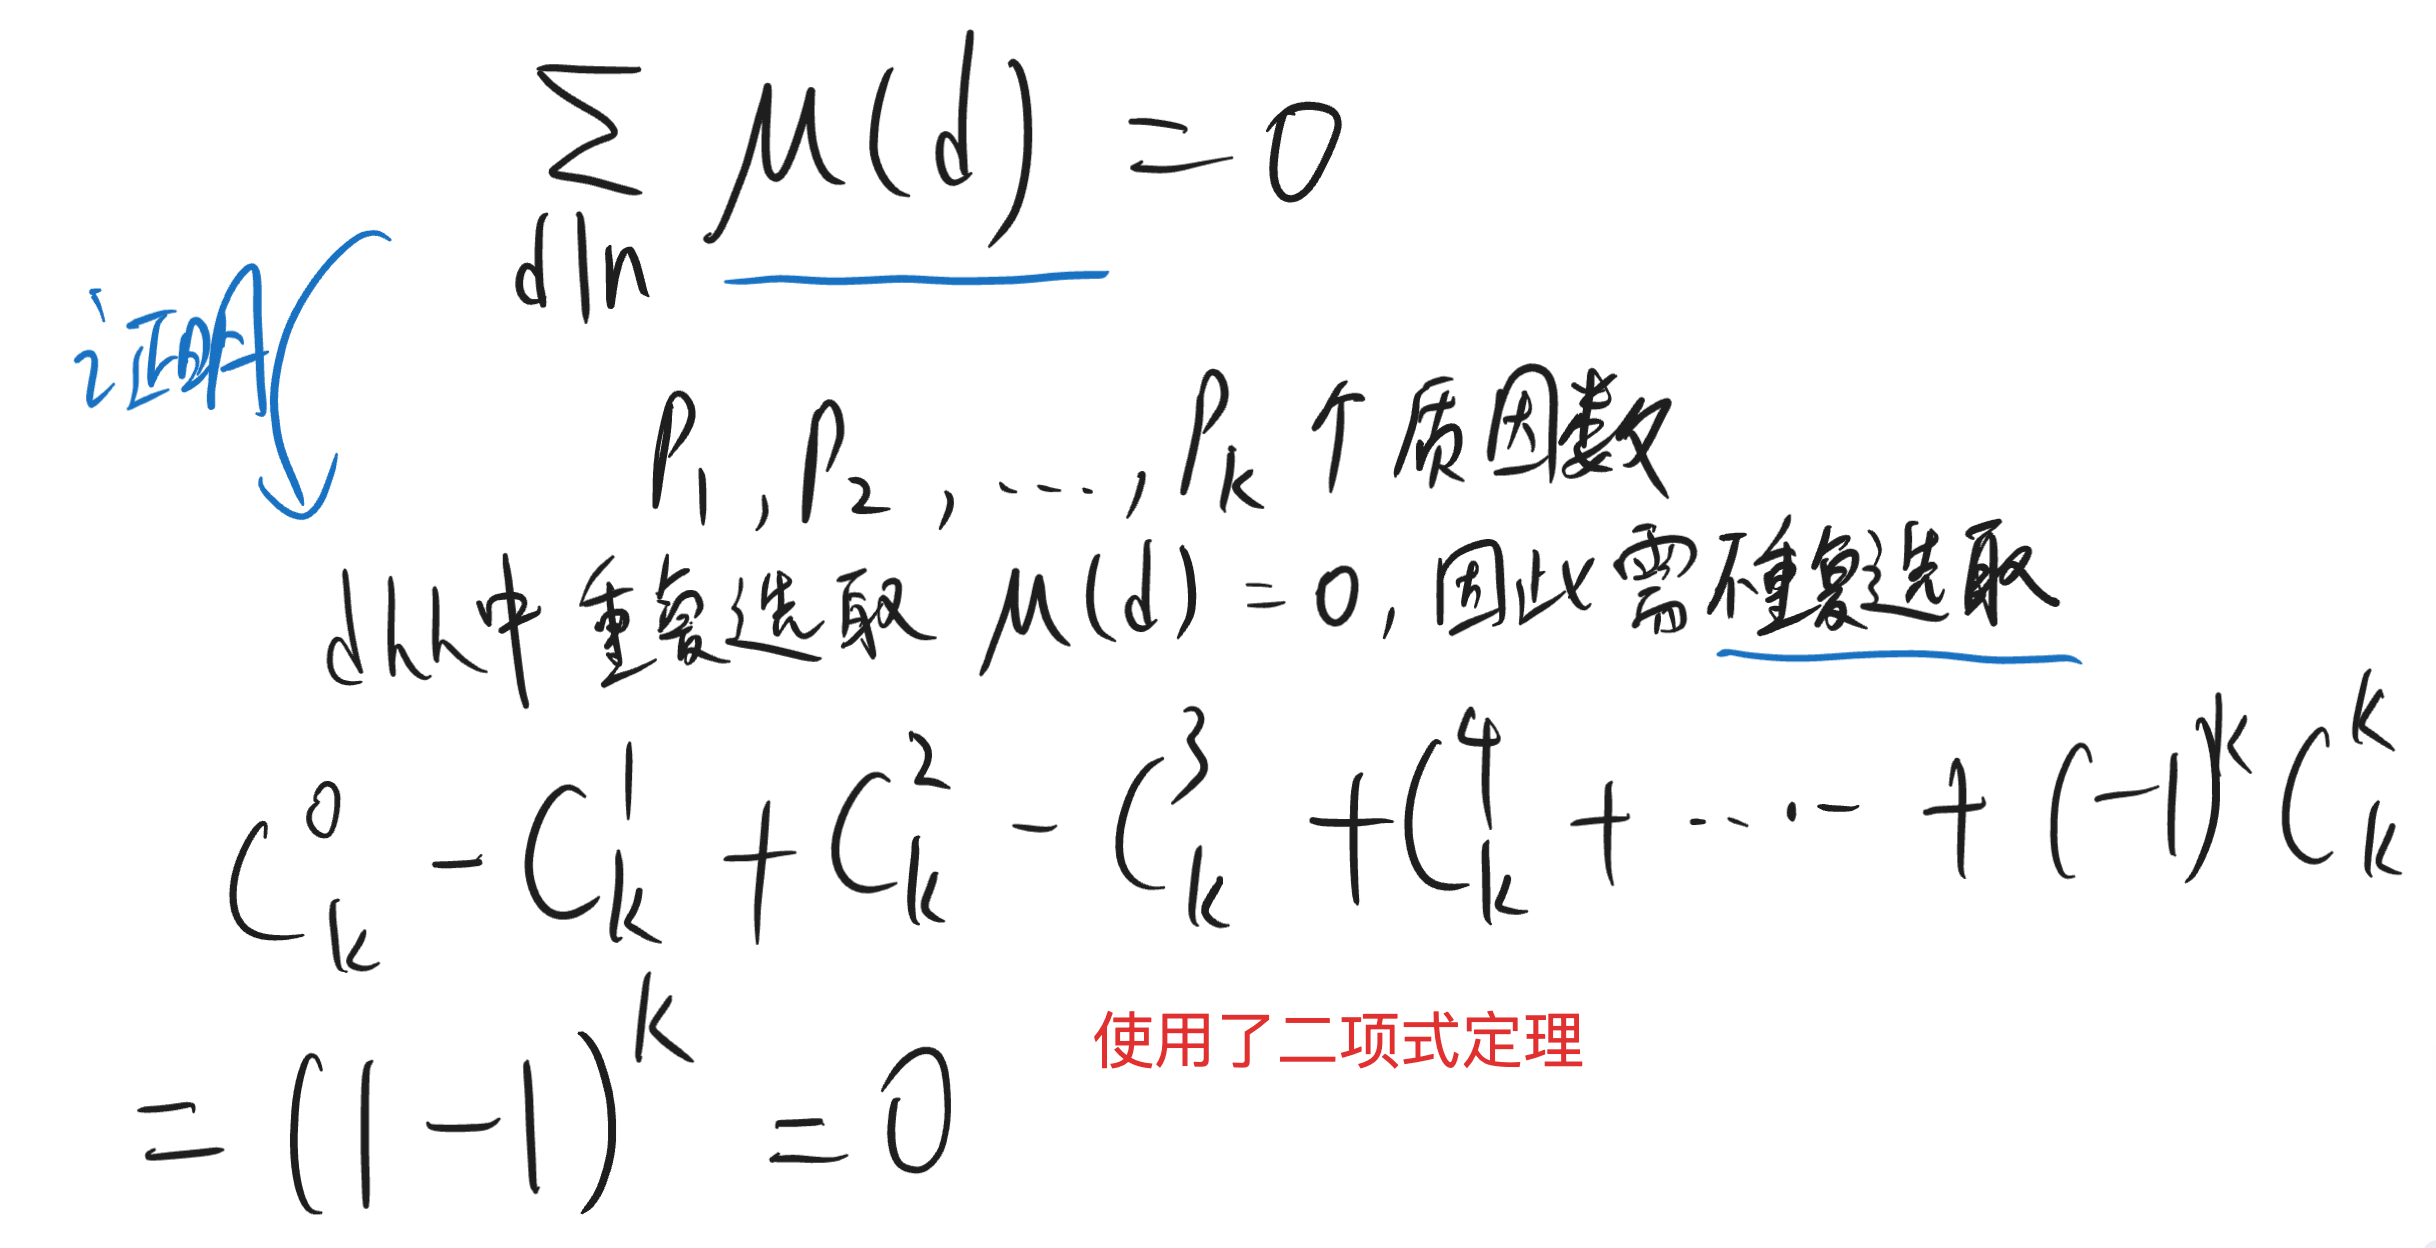
\includegraphics[width=0.92\linewidth]{image/mobius_proof_3_lemma.png}
	\end{center}

	\subsubsection{反演公式（因数形式）的证明}

	\textbf{命题.} 已知 $f(n)=\sum_{d\mid n}g(d)$，要证 $g(n)=\sum_{d\mid n}\mu(n/d)\,f(d)$：

	\begin{center}
		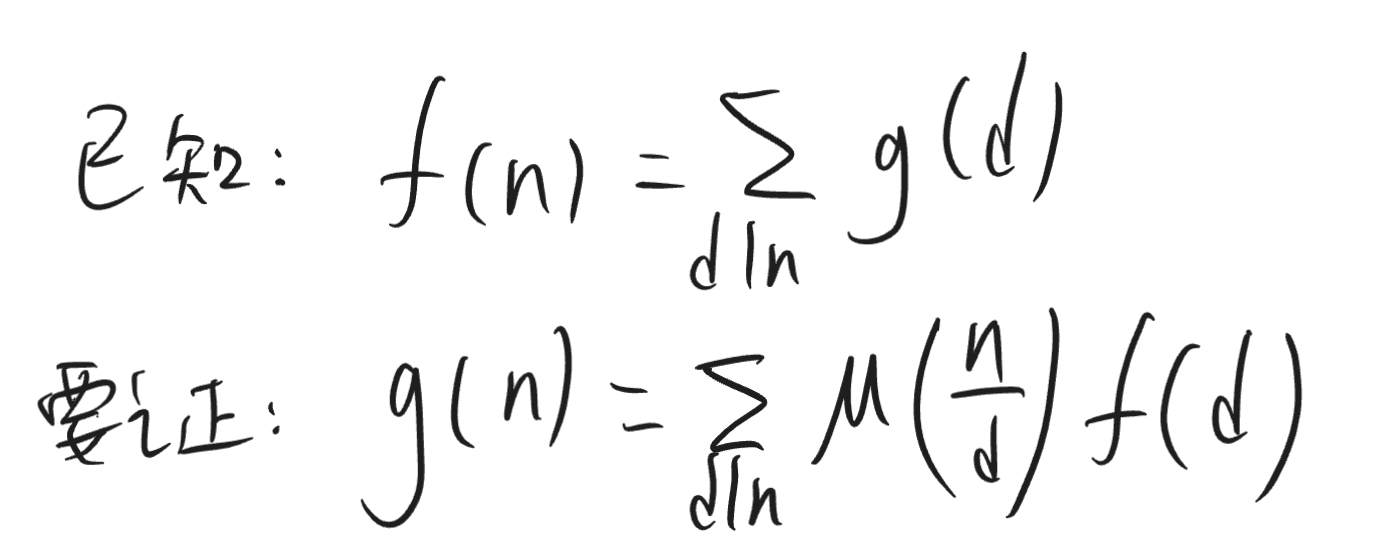
\includegraphics[width=0.72\linewidth]{image/mobius_proof_1_statement.png}
	\end{center}

	\textbf{代入并交换求和次序.} 把右边的 $f(d)$ 代入为 $\sum_{k\mid d}g(k)$，交换求和次序后令 $x=n/d$，内层中括号化为 $\sum_{x\mid n/k}\mu(x)$：

	\begin{center}
		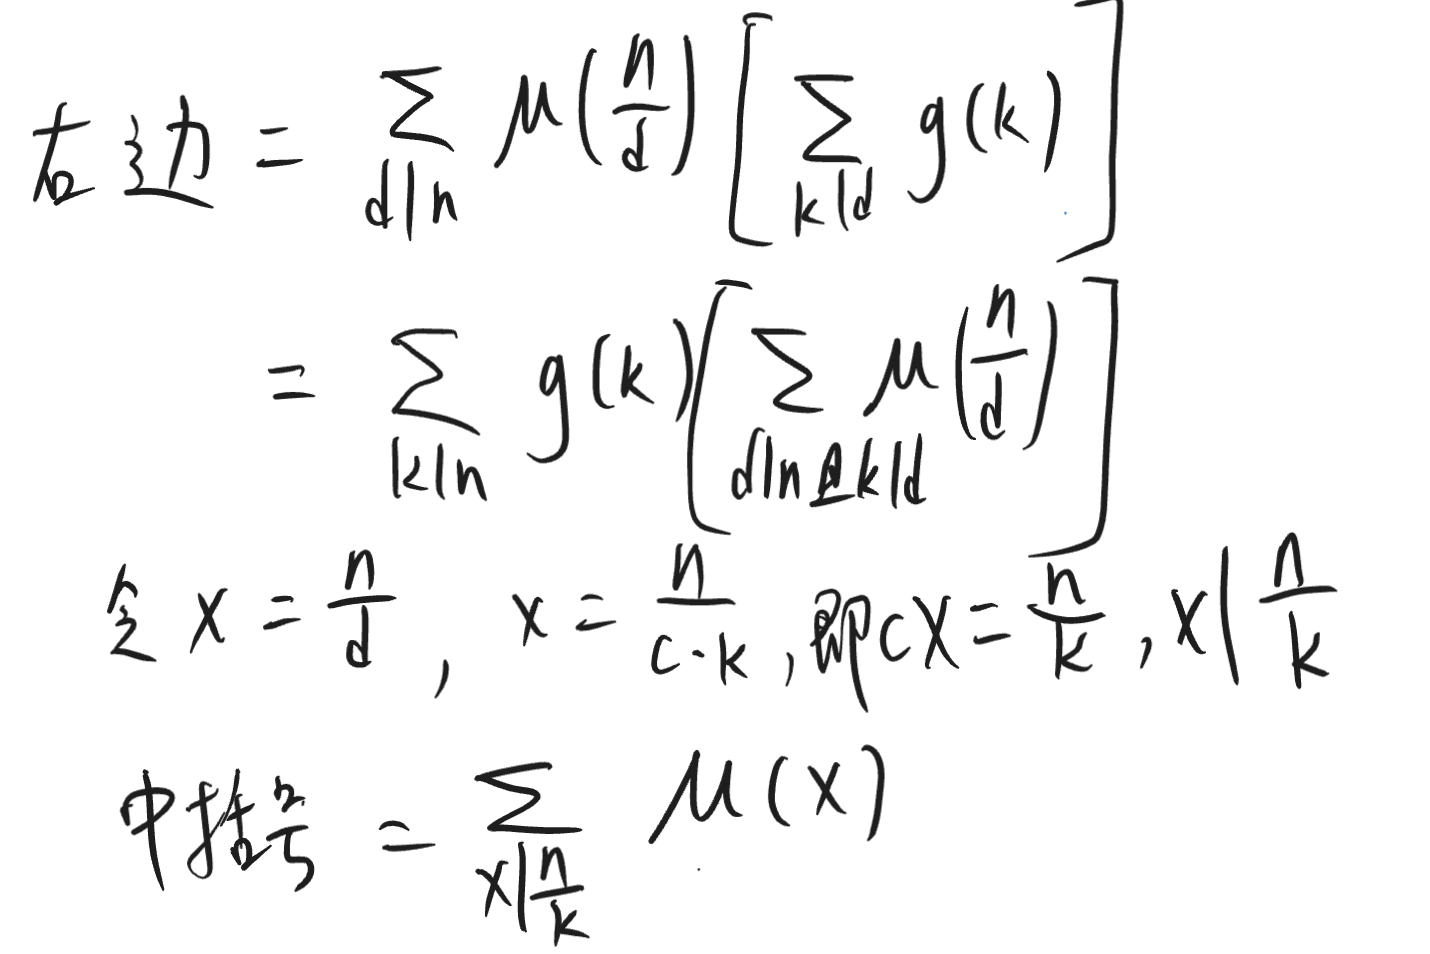
\includegraphics[width=0.80\linewidth]{image/mobius_proof_2_swap.png}
	\end{center}

	\textbf{用 $\mu$ 的性质收束.} 由关键引理 $\sum_{x\mid n/k}\mu(x)=[\,n/k=1\,]=[\,k=n\,]$，于是右边 $=\sum_{k\mid n}g(k)\,[\,k=n\,]=g(n)=$ 左边，得证：

	\begin{center}
		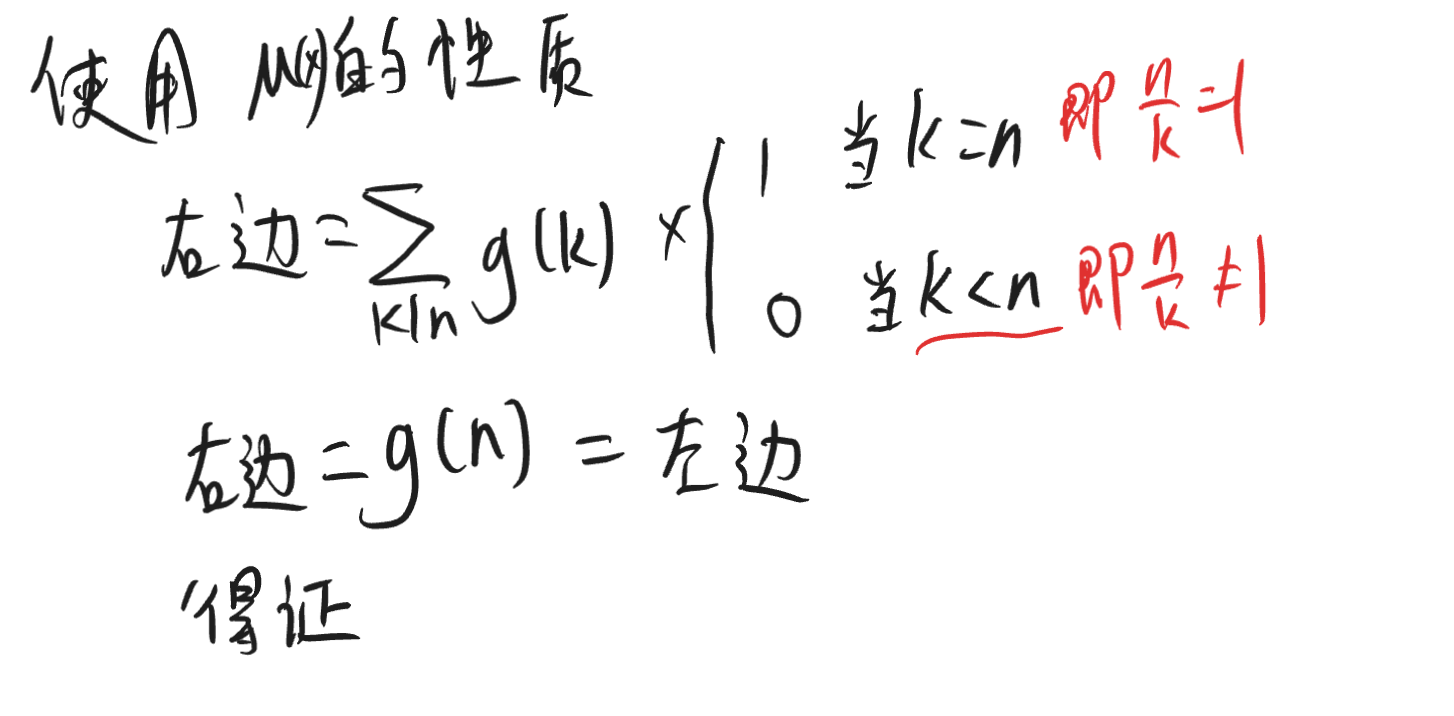
\includegraphics[width=0.82\linewidth]{image/mobius_proof_4_finish.png}
	\end{center}

	\textbf{求和次序交换示意（$n=12$）.} 上面「交换求和次序」一步，可用约数 incidence 网格直观理解——原式与交换后覆盖的是同一批 $(k,d)$ 点对：

	\begin{center}
	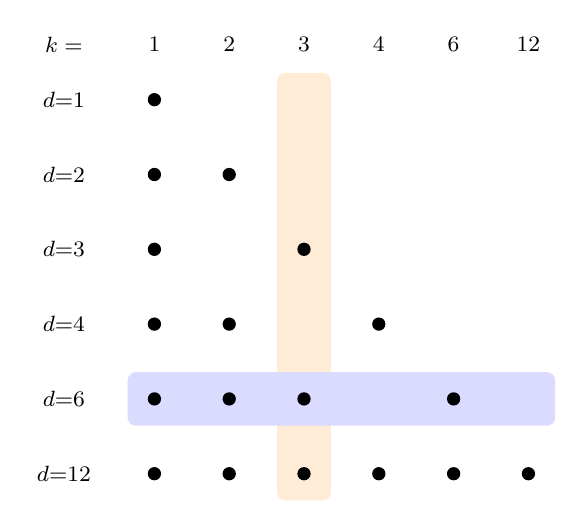
\begin{tikzpicture}[scale=1.0]
		% 12 的约数：k 作列（横轴），d 作行（纵轴，自上而下）
		% D = {1,2,3,4,6,12}，索引 0..5
		% 列高亮：k=3（第 2 列，j=2）——固定 k、纵向对 d 求和
		\fill[orange!16, rounded corners=3pt] (2*0.95-0.34, 0.34) rectangle (2*0.95+0.34, -5*0.95-0.34);
		% 行高亮：d=6（第 4 行，i=4）——固定 d、横向对 k 求和
		\fill[blue!14, rounded corners=3pt] (-0.34, -4*0.95+0.34) rectangle (5*0.95+0.34, -4*0.95-0.34);

		% 列标题 k
		\foreach \j/\kv in {0/1,1/2,2/3,3/4,4/6,5/12}
			\node[font=\footnotesize] at (\j*0.95, 0.7) {$\kv$};
		\node[font=\footnotesize] at (-1.15, 0.7) {$k=$};
		% 行标题 d
		\foreach \i/\dv in {0/1,1/2,2/3,3/4,4/6,5/12}
			\node[font=\footnotesize] at (-1.15, -\i*0.95) {$d{=}\dv$};

		% 每个 k | d 的格子画实心点（incidence）
		\foreach \i/\js in {0/{0}, 1/{0,1}, 2/{0,2}, 3/{0,1,3}, 4/{0,1,2,4}, 5/{0,1,2,3,4,5}}
			\foreach \j in \js
				\fill[black] (\j*0.95, -\i*0.95) circle (2.4pt);
	\end{tikzpicture}

	{\footnotesize 求和次序交换（$n=12$，约数 $\{1,2,3,4,6,12\}$）：实心点表示 $k \mid d$。\textcolor{blue}{蓝行}是原式「固定 $d=6$、横向对 $k \mid d$ 求和」；\textcolor{orange}{橙列}是交换后「固定 $k=3$、纵向对满足 $k \mid d \mid n$ 的 $d$ 求和」。两种方式覆盖的是同一批点，故可交换。}
	\end{center}
